\documentclass[12pt,a4paper]{report}
\usepackage[utf8]{inputenc}
\usepackage[T1]{fontenc}
\usepackage{lmodern}
\usepackage[a4paper,margin=1in]{geometry}
\usepackage{setspace,graphicx,array,booktabs,longtable,enumitem,xcolor,hyperref,listings,tikz,fancyhdr}
\usetikzlibrary{arrows.meta,positioning,shapes.geometric}
\onehalfspacing
\hypersetup{colorlinks=true,linkcolor=blue,urlcolor=blue,pdftitle={Online Voting System for Class Representatives}}
\pagestyle{fancy}\fancyhf{}\lhead{ICT Lab -- CL-1000}\rhead{Online Voting System}\cfoot{\thepage}
\definecolor{codeblue}{RGB}{25,55,100}
\lstset{basicstyle=\ttfamily\small,keywordstyle=\color{codeblue}\bfseries,commentstyle=\color{gray}\itshape,stringstyle=\color{red!65!black},numbers=left,numberstyle=\tiny\color{gray},breaklines=true,frame=single,showstringspaces=false,tabsize=2}
\begin{document}
\begin{titlepage}\centering
\vspace*{1cm}
{\Large\textbf{National University of Computer and Emerging Sciences}}\\[0.3cm]
{\large Karachi Campus}\\[0.8cm]
{\large Introduction to Information and Communication Technology Lab}\\
{\large CL-1000 \;|\; Fall 2026}\\[1.2cm]
\rule{\textwidth}{1.2pt}\\[0.4cm]
{\Huge\textbf{Project Report}}\\[0.3cm]
{\LARGE\textbf{Online Voting System for Class Representatives}}\\[0.4cm]
\rule{\textwidth}{1.2pt}\\[1.2cm]
\begin{tabular}{>{\bfseries}p{4cm}p{8cm}}
Course Section: & BDS-1B\\
Instructor: & Ms. Saira Ayub\\
Group Member 1: & Kishore Kumar (26K-2554)\\
Group Member 2: & Mohammad Asher Musdasir (26K-2531)\\
Group Member 3: & Ali Hadi (26K-2538)\\
Proposal Date: & 22 October 2026\\
Report Date: & \today
\end{tabular}
\vfill{\large\textbf{ICT Lab Project}}
\end{titlepage}
\pagenumbering{roman}\tableofcontents\listoffigures\clearpage\pagenumbering{arabic}

\chapter*{Abstract}\addcontentsline{toc}{chapter}{Abstract}
The Online Voting System for Class Representatives is a proposed web-based application designed to make small class elections more organized and efficient. Instead of paper ballots or manual counting, eligible students log in using a roll number and password, view candidates, and submit one vote. The system records the vote, prevents repeat submissions within the defined process, and calculates results automatically. The planned tools are HTML, CSS, JavaScript, and MS Excel. This report describes the problem, objectives, requirements, technologies, workflow, proposed algorithms, testing, limitations, and future improvements.
\textbf{Keywords:} Online voting, class representative, HTML, CSS, JavaScript, MS Excel.

\chapter{Introduction}
\section{Project Overview}
The Online Voting System for Class Representatives is intended to provide a simple digital method for students to elect their class representatives. Students use a web interface to log in, view the available candidates, and cast a vote. The system checks eligibility and voting status, records the submitted vote, and displays results after the election closes. It is designed for small classroom elections to save time, reduce manual effort, and organize the process.
\section{Background}
Class representatives communicate students' concerns and information between the class and the teacher or department. Selecting a representative is an important classroom activity. Traditional methods such as raising hands or paper slips can take time and require manual counting. A digital process can make the activity more structured.
\section{Purpose}
This report documents the proposed system and explains its expected modules and workflow. It can guide development, demonstration, and evaluation.

\chapter{Problem Statement and Objectives}
\section{Problem Statement}
In many classes, representatives are selected by raising hands or using paper slips. These methods can waste class time, may be influenced by peer pressure, and can lead to votes being miscounted, lost, or submitted more than once. Students absent on election day may miss the opportunity to participate. The proposed system addresses these issues through an online platform where a verified student can vote once, privately, within a fixed election period, and where results are counted automatically.
\section{Objectives}
\begin{enumerate}
\item Design a user-friendly platform where students can view candidates and cast a vote.
\item Verify eligible students using roll number and password.
\item Prevent a student from submitting more than one vote.
\item Keep the voting process private and handle vote records carefully.
\item Count votes automatically and display the final result.
\item Reduce time, paperwork, and manual errors in class elections.
\end{enumerate}
\section{Scope}
The initial scope is limited to class representative elections. It includes an administrator-managed student list and candidate list, student login, one-vote submission, vote recording, and result calculation. The proposal does not define a large-scale public election platform.

\chapter{System Requirements}
\section{Functional Requirements}
\begin{enumerate}
\item Administrator maintains the eligible student list.
\item Administrator enters the candidate list.
\item Student logs in using roll number and password.
\item System verifies the student's details.
\item System checks whether the student has already voted.
\item Eligible student selects one candidate and submits a vote.
\item System records the vote and marks the student as voted.
\item System displays a confirmation message.
\item After the election closes, the system calculates and displays vote totals.
\end{enumerate}
\section{Non-Functional Requirements}
\begin{itemize}
\item \textbf{Usability:} Pages should be simple and understandable.
\item \textbf{Accessibility:} Interface should work on common screen sizes.
\item \textbf{Reliability:} Valid and invalid inputs should be handled consistently.
\item \textbf{Performance:} Login checks and result calculations should be quick for a small class.
\item \textbf{Privacy:} Individual students' choices should not be publicly revealed.
\item \textbf{Maintainability:} HTML, CSS, and JavaScript should be organized clearly.
\end{itemize}
\section{System Users}
\textbf{Administrator:} The class teacher or election committee member who maintains students, candidates, and election status.\\
\textbf{Student/Voter:} An eligible student who logs in and submits one vote.

\chapter{Tools and Technologies}
\section{HTML}
HTML (HyperText Markup Language) creates the structure of the website, including login, candidate, voting, and results pages.
\section{CSS}
CSS (Cascading Style Sheets) styles the pages by controlling layout, colors, spacing, typography, and responsive presentation.
\section{JavaScript}
JavaScript provides browser-side interaction. It is intended to validate form inputs, support voting actions, check voting status in the prototype, and calculate or display results based on available vote records.
\section{MS Excel}
MS Excel is proposed for maintaining the student list, candidate data, and final result records for verification. The team should document how website data is transferred to or checked against the spreadsheet.
\section{Why These Technologies}
These tools are beginner-friendly and commonly available. HTML, CSS, and JavaScript run in a browser, while Excel can maintain and review small sets of class data.
\textbf{Implementation note:} The proposal identifies Excel as a record and verification tool, but does not specify a live database or secure server. A browser-only demonstration should be described as an academic prototype. Client-side checks alone are not sufficient to secure a real election.

\chapter{System Design}
\section{High-Level Architecture}
The proposed system has three areas:
\begin{enumerate}
\item \textbf{Presentation layer:} HTML pages and CSS styling shown in the browser.
\item \textbf{Interaction layer:} JavaScript for form validation, voting actions, and result presentation.
\item \textbf{Record-keeping:} Student, candidate, and result records maintained through the planned Excel workflow.
\end{enumerate}
\section{Main Modules}
\subsection{Administrator Module}
The administrator prepares the election by entering eligible students and candidates and setting the election period.
\subsection{Student Login Module}
The student enters a roll number and password. The system checks whether the details match an eligible student record.
\subsection{Candidate Display Module}
After successful login, the student views the available candidates and their details.
\subsection{Voting Module}
The student selects one candidate and submits the vote. The system checks voting status and accepts no more than one vote from a student within the prototype's defined process.
\subsection{Result Module}
After the election closes, the system counts recorded votes for each candidate and displays the totals and winner.

\chapter{Project Workflow}
\section{Step-by-Step Workflow}
\begin{enumerate}
\item Administrator creates the election and enters candidates.
\item Administrator prepares the eligible student list.
\item Student opens the website and logs in using roll number and password.
\item System verifies the student's details.
\item System checks whether the student has already voted.
\item If eligible and not previously voted, the candidate list is displayed.
\item Student selects one candidate and submits the vote.
\item System records the vote and marks the student as voted.
\item A confirmation message is displayed.
\item After the election closes, votes are counted and results are displayed.
\end{enumerate}
\section{Workflow Diagram}
\begin{figure}[htbp]\centering
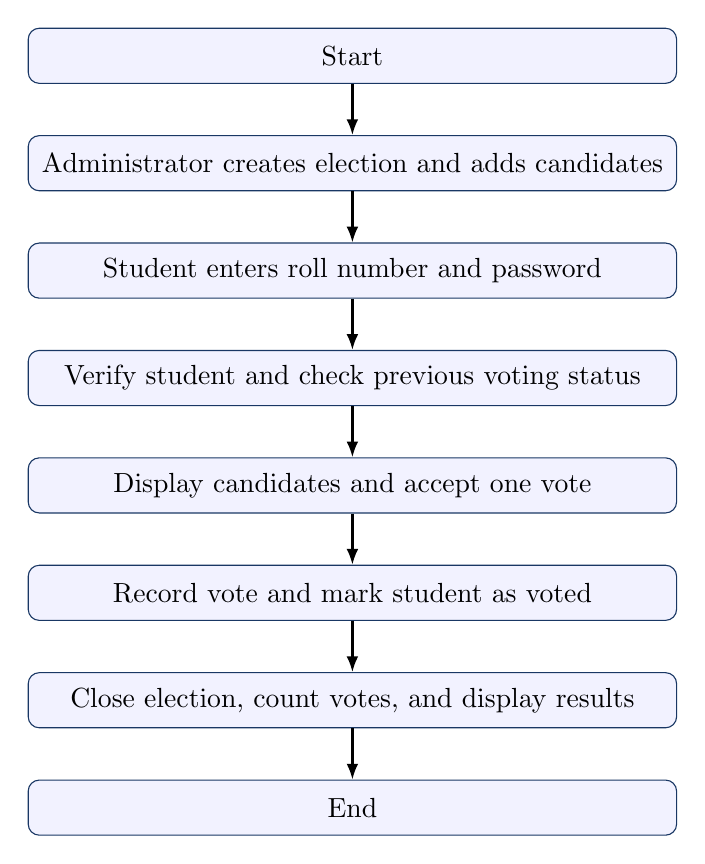
\begin{tikzpicture}[node distance=0.65cm,process/.style={rectangle,rounded corners,draw=codeblue,fill=blue!5,text width=8cm,align=center,minimum height=0.7cm},arrow/.style={-{Latex[length=2mm]},thick}]
\node[process] (a) {Start};
\node[process,below=of a] (b) {Administrator creates election and adds candidates};
\node[process,below=of b] (c) {Student enters roll number and password};
\node[process,below=of c] (d) {Verify student and check previous voting status};
\node[process,below=of d] (e) {Display candidates and accept one vote};
\node[process,below=of e] (f) {Record vote and mark student as voted};
\node[process,below=of f] (g) {Close election, count votes, and display results};
\node[process,below=of g] (h) {End};
\draw[arrow](a)--(b);\draw[arrow](b)--(c);\draw[arrow](c)--(d);\draw[arrow](d)--(e);\draw[arrow](e)--(f);\draw[arrow](f)--(g);\draw[arrow](g)--(h);
\end{tikzpicture}
\caption{Proposed workflow of the Online Voting System}
\end{figure}

\chapter{Proposed Algorithms}
The following language-independent outlines describe the expected logic; they do not claim that a complete secure backend has already been implemented.
\section{Login Verification}
\begin{lstlisting}
INPUT rollNumber, password
FIND student record using rollNumber

IF no matching student exists
    DISPLAY "Invalid student details"
ELSE IF password does not match
    DISPLAY "Invalid student details"
ELSE
    CONTINUE to voting-status check
END IF
\end{lstlisting}
\section{One-Vote Check and Submission}
\begin{lstlisting}
IF student has already voted
    DISPLAY "You have already submitted your vote"
ELSE
    DISPLAY candidate list
    GET selected candidate
    VALIDATE selected candidate
    SAVE vote record
    MARK student as voted
    DISPLAY confirmation message
END IF
\end{lstlisting}
\section{Automatic Vote Counting}
\begin{lstlisting}
FOR each candidate
    candidateVoteCount = 0
    FOR each recorded vote
        IF vote belongs to candidate
            candidateVoteCount = candidateVoteCount + 1
        END IF
    END FOR
    DISPLAY candidate name and candidateVoteCount
END FOR
DISPLAY candidate with the highest vote total
\end{lstlisting}

\chapter{Proposed User Interface}
The website is expected to contain these pages:
\begin{enumerate}
\item \textbf{Login Page:} Fields for roll number and password.
\item \textbf{Candidate Page:} List of candidates participating in the election.
\item \textbf{Voting Page:} Allows the student to select one candidate and submit a vote.
\item \textbf{Confirmation Page:} Confirms successful vote submission.
\item \textbf{Results Page:} Displays candidate names and vote totals after the election closes.
\item \textbf{Administrator Page:} Maintains the student list, candidate list, and election status.
\end{enumerate}

\chapter{Testing and Validation}
The following test cases should be run during development. Fill in the actual result column after testing the application.
\begin{longtable}{p{0.7cm}p{4.3cm}p{5.3cm}p{2.4cm}}
\toprule
\textbf{No.}&\textbf{Test Case}&\textbf{Expected Result}&\textbf{Actual Result}\\\midrule
1&Enter valid student login details.&Student proceeds to voting area.&To be tested\\
2&Enter an unknown roll number.&System rejects the login.&To be tested\\
3&Enter an incorrect password.&System rejects the login.&To be tested\\
4&Submit a vote as an eligible student.&Vote is recorded and confirmation appears.&To be tested\\
5&Try to vote a second time.&System blocks the second submission.&To be tested\\
6&Submit without selecting a candidate.&System asks the student to select a candidate.&To be tested\\
7&Close election and open results.&Vote totals are calculated and displayed.&To be tested\\
8&Compare displayed totals with recorded votes.&Totals match the records.&To be tested\\
\bottomrule
\end{longtable}

\chapter{Security Considerations and Limitations}
\section{Security Considerations}
The proposed system aims to verify students and prevent repeat voting. A reliable real-world voting system needs more than browser-side validation. A production version should use a trusted server, secure authentication, protected storage, administrator access control, and audit logs. It should also separate voter identity from ballot choice so individual choices remain private.
\section{Current Limitations}
\begin{itemize}
\item The project is intended for a small classroom election.
\item The proposal does not define a server-side database or deployment platform.
\item Excel is proposed for maintaining and checking records; it is not described as a live multi-user database.
\item Browser-side JavaScript alone cannot guarantee one-vote-per-person against deliberate manipulation.
\item Actual functionality must be verified through project testing.
\end{itemize}

\chapter{Future Enhancements}
\begin{enumerate}
\item Add a server-side database for student, candidate, and vote records.
\item Add stronger authentication and password protection.
\item Provide a dedicated administrator dashboard.
\item Add election start and end time controls.
\item Improve privacy by separating voter authentication records from ballot choices.
\item Add downloadable result reports and turnout summaries.
\item Improve the interface for mobile phones and tablets.
\item Add audit and backup features to help verify final results.
\end{enumerate}

\chapter{Conclusion}
The Online Voting System for Class Representatives is an ICT project intended to improve small class elections through a structured digital workflow. Students are expected to log in, view candidates, and submit one vote, while the system records votes and calculates results automatically. HTML, CSS, JavaScript, and MS Excel are the planned tools for building and demonstrating the initial class-level prototype. Future versions can be improved through server-side storage, stronger security, and better privacy controls.

\begin{thebibliography}{9}
\bibitem{html} WHATWG, \textit{HTML Living Standard}. \url{https://html.spec.whatwg.org/}
\bibitem{css} W3C, \textit{CSS Specifications}. \url{https://www.w3.org/Style/CSS/}
\bibitem{js} MDN Web Docs, \textit{JavaScript Guide}. \url{https://developer.mozilla.org/en-US/docs/Web/JavaScript/Guide}
\bibitem{excel} Microsoft Support, \textit{Excel Help and Learning}. \url{https://support.microsoft.com/excel}
\end{thebibliography}
\end{document}